\documentclass[12pt,a4paper]{article}
\usepackage[utf8]{vietnam}
\usepackage{amsmath,amssymb}
\usepackage{tabularx}
\usepackage{tikz}
\usetikzlibrary{calc,arrows.meta}
\usepackage{xcolor}
\usepackage{enumitem}
\usepackage{fancyhdr}
\usepackage[top=1.2cm, bottom=1.2cm, left=1.5cm, right=1.5cm]{geometry}
\usepackage[loigiai]{ex_test}
\SAOPTN{widthSA=2.6,heightSA=0.62}

\setlength{\headheight}{15pt}
\setlength{\parskip}{0pt}

\pagestyle{fancy}
\fancyhf{}
\rhead{\textit{Lời giải chi tiết -- Đề số 6}}
\lhead{\textit{Bộ đề ôn tập Giữa học kì I -- Toán 7}}
\cfoot{\thepage}

\begin{document}

\begin{center}
\textbf{\Large HƯỚNG DẪN CHẤM VÀ LỜI GIẢI CHI TIẾT}\\
\vspace{1.5mm}
\textbf{\large MÔN: TOÁN 7 -- ĐỀ SỐ 6}
\end{center}
\vspace{2mm}

\noindent\textbf{\large PHẦN I. CÂU TRẮC NGHIỆM NHIỀU PHƯƠNG ÁN LỰA CHỌN}

\vspace{1mm}
\begin{ex}
Tập hợp các số hữu tỉ được ký hiệu là:
\choice
{$\mathbb{N}$}
{$\mathbb{Z}$}
{\True $\mathbb{Q}$}
{$\mathbb{R}$}
\loigiai{
Tập hợp các số hữu tỉ được ký hiệu bằng chữ cái $\mathbb{Q}$.
}
\end{ex}

\begin{ex}
Kết quả của phép tính $4^3 \cdot 4^9$ bằng:
\choice
{$4^6$}
{$4^3$}
{\True $4^{12}$}
{$2^{27}$}
\loigiai{
Áp dụng quy tắc nhân hai lũy thừa cùng cơ số $a^m \cdot a^n = a^{m+n}$:
\[ 4^3 \cdot 4^9 = 4^{3+9} = 4^{12}. \]
}
\end{ex}

\begin{ex}
\immini{
Cho hình vẽ sau. Kết luận nào sau đây SAI?
\choice
{$a \parallel b$}
{$c \perp b$}
{$c \perp a$}
{\True $a \perp b$}
}{
\begin{tikzpicture}[scale=0.9, line cap=round, line join=round]
    \draw[thick, blue!70!black] (-2.2, 1.5) -- (3.5, 1.5) node[above=2pt] {$a$};
    \draw[thick, blue!70!black] (-2.2, 0) -- (3.5, 0) node[below=2pt] {$b$};
    \draw[thick, blue!70!black] (0, 2.3) node[above right=1pt] {$c$} -- (0, -0.8);
    \draw[thick, blue!70!black] (0, 1.5) rectangle +(0.32, 0.32);
    \draw[thick, blue!70!black] (0, 0) rectangle +(0.32, 0.32);
\end{tikzpicture}
}
\loigiai{
Từ hình vẽ ta thấy $c \perp a$ và $c \perp b$, do đó khẳng định B và C đúng.
Hai đường thẳng phân biệt cùng vuông góc với một đường thẳng thứ ba thì song song với nhau, suy ra $a \parallel b$ (khẳng định A đúng).
Khẳng định D: $a \perp b$ là SAI.
}
\end{ex}

\begin{ex}
Hình hộp chữ nhật có tất cả bao nhiêu mặt?
\choice
{$2$}
{$4$}
{\True $6$}
{$8$}
\loigiai{
Hình hộp chữ nhật có tất cả 6 mặt, gồm 2 mặt đáy và 4 mặt bên.
}
\end{ex}

\begin{ex}
Với $a, b, c$ là ba số hữu tỉ bất kì, nếu $a - b = c$ thì:
\choice
{\True $a = c + b$}
{$a = -b + c$}
{$a = b - c$}
{$a = -b - c$}
\loigiai{
Theo quy tắc chuyển vế, khi chuyển $-b$ từ vế trái sang vế phải ta đổi dấu thành $+b$:
\[ a - b = c \implies a = c + b. \]
}
\end{ex}

\begin{ex}
Hãy so sánh hai số hữu tỉ $-0{,}2$ và $-\dfrac{2}{5}$:
\choice
{$-0{,}2 < -\dfrac{2}{5}$}
{\True $-0{,}2 > -\dfrac{2}{5}$}
{$-0{,}2 = -\dfrac{2}{5}$}
{$-0{,}2 \ge -\dfrac{2}{5}$}
\loigiai{
Ta đổi phân số $-\dfrac{2}{5}$ về số thập phân: $-\dfrac{2}{5} = -0{,}4$.
Vì $0{,}2 < 0{,}4$ nên $-0{,}2 > -0{,}4$, tức là $-0{,}2 > -\dfrac{2}{5}$.
}
\end{ex}

\begin{ex}
Giá trị của $|-3|$ bằng:
\choice
{$-3$}
{\True $3$}
{$\dfrac{1}{3}$}
{$-\dfrac{1}{3}$}
\loigiai{
Giá trị tuyệt đối của một số luôn không âm. Vì $-3 < 0$ nên $|-3| = -(-3) = 3$.
}
\end{ex}

\begin{ex}
Căn bậc hai số học của $49$ là:
\choice
{$-7$}
{\True $7$}
{$-7$ và $7$}
{$-49$}
\loigiai{
Căn bậc hai số học của số $a \ge 0$ là số không âm $\sqrt{a}$.
Do $7 > 0$ và $7^2 = 49$ nên căn bậc hai số học của $49$ là $7$.
}
\end{ex}

\begin{ex}
Trong các số sau, số nào là số vô tỉ?
\choice
{$\sqrt{25}$}
{\True $\sqrt{3}$}
{$(3{,}5)^2$}
{$\sqrt{16}$}
\loigiai{
Ta có $\sqrt{25} = 5$ (số hữu tỉ), $(3{,}5)^2 = 12{,}25$ (số hữu tỉ), $\sqrt{16} = 4$ (số hữu tỉ).
Số $\sqrt{3} \approx 1{,}73205\dots$ là số thập phân vô hạn không tuần hoàn nên $\sqrt{3}$ là số vô tỉ.
}
\end{ex}

\begin{ex}
Kết quả của phép tính $-\dfrac{3}{20} + \left(-\dfrac{2}{15}\right)$ là:
\choice
{$-\dfrac{1}{35}$}
{\True $-\dfrac{17}{60}$}
{$-\dfrac{5}{35}$}
{$-\dfrac{1}{60}$}
\loigiai{
Quy đồng mẫu số chung là $60$:
\[ -\dfrac{3}{20} + \left(-\dfrac{2}{15}\right) = -\dfrac{9}{60} - \dfrac{8}{60} = -\dfrac{17}{60}. \]
}
\end{ex}

\begin{ex}
\immini{
Cho hình vẽ sau, biết $a \parallel b, \widehat{A} = 45^\circ$. Số đo của $\widehat{B}_1$ bằng bao nhiêu?
\choice
{$145^\circ$}
{$45^\circ$}
{$35^\circ$}
{\True $135^\circ$}
}{
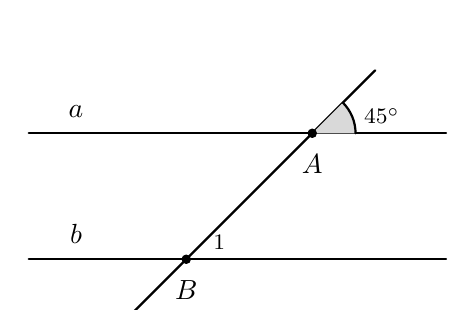
\begin{tikzpicture}[scale=1.0, line cap=round, line join=round]
    \coordinate (B) at (1.2, 0);
    \coordinate (A) at (2.8, 1.6);
    \draw[thick] (-0.8, 1.6) -- (4.5, 1.6);
    \node[above=2pt] at (-0.2, 1.6) {$a$};
    \draw[thick] (-0.8, 0) -- (4.5, 0);
    \node[above=2pt] at (-0.2, 0) {$b$};
    \draw[thick] ($(A)!1.5!(B)$) -- ($(B)!1.5!(A)$);
    \fill[gray!30] (A) -- ++(0:0.55) arc (0:45:0.55) -- cycle;
    \draw[thick] (A) ++(0:0.55) arc (0:45:0.55);
    \node[font=\footnotesize, right=1pt] at ($(A)+(0.5, 0.22)$) {$45^\circ$};
    \filldraw[black] (A) circle (1.5pt) node[below=4pt] {$A$};
    \filldraw[black] (B) circle (1.5pt) node[below=4pt] {$B$};
    \node[font=\footnotesize] at ($(B)+(0.42, 0.22)$) {$1$};
\end{tikzpicture}
}
\loigiai{
Dựa vào hình vẽ, góc cho trước $45^\circ$ và góc $\widehat{B}_1$ ở vị trí kề bù với góc đồng vị $45^\circ$ (hoặc hai góc trong cùng phía bù nhau):
\[ \widehat{B}_1 = 180^\circ - 45^\circ = 135^\circ. \]
}
\end{ex}

\begin{ex}
Điền cụm từ thích hợp vào chỗ trống: ''Qua một điểm nằm ngoài đường thẳng \dots đường thẳng song song với đường thẳng đó''.
\choice
{có vô số}
{\True chỉ có một}
{có hai}
{có ba}
\loigiai{
Theo tiên đề Euclid: ''Qua một điểm nằm ngoài một đường thẳng chỉ có một đường thẳng song song với đường thẳng đó''.
}
\end{ex}


\setcounter{ex}{0}
\noindent\textbf{\large PHẦN II. CÂU TRẮC NGHIỆM ĐÚNG SAI}

\vspace{1mm}
\begin{ex}
Cho biểu thức $A = \dfrac{3}{4} - \dfrac{1}{2} \cdot \left(-\dfrac{2}{3}\right)$ và $B = \left|-\dfrac{5}{6}\right|$. Xét tính đúng sai của các mệnh đề sau:
\choiceTF
{\True Giá trị của phép tính $\dfrac{1}{2} \cdot \left(-\dfrac{2}{3}\right)$ bằng $-\dfrac{1}{3}$}
{\True Giá trị của biểu thức $A$ bằng $\dfrac{13}{12}$}
{\True Giá trị của $B$ bằng $\dfrac{5}{6}$}
{Hiệu $A - B$ là một số hữu tỉ âm}
\loigiai{
\begin{itemize}[leftmargin=0.5cm, itemsep=1pt]
\item \textbf{a)} \textbf{Đúng}. Ta có $\dfrac{1}{2} \cdot \left(-\dfrac{2}{3}\right) = \dfrac{1 \cdot (-2)}{2 \cdot 3} = -\dfrac{1}{3}$.
\item \textbf{b)} \textbf{Đúng}. Ta có $A = \dfrac{3}{4} - \left(-\dfrac{1}{3}\right) = \dfrac{3}{4} + \dfrac{1}{3} = \dfrac{9}{12} + \dfrac{4}{12} = \dfrac{13}{12}$.
\item \textbf{c)} \textbf{Đúng}. Giá trị tuyệt đối của số âm là số đối của nó: $B = \left|-\dfrac{5}{6}\right| = \dfrac{5}{6}$.
\item \textbf{d)} \textbf{Sai}. Ta có $A - B = \dfrac{13}{12} - \dfrac{5}{6} = \dfrac{13}{12} - \dfrac{10}{12} = \dfrac{3}{12} = \dfrac{1}{4} > 0$. Do đó $A - B$ là một số hữu tỉ dương.
\end{itemize}
}
\end{ex}

\begin{ex}
Cho hai đường thẳng $xy$ và $zt$ song song với nhau. Đường thẳng $mn$ cắt $xy$ tại $M$ và cắt $zt$ tại $N$. Biết số đo góc $\widehat{xMN} = 55^\circ$. Xét tính đúng sai của các mệnh đề sau:
\choiceTF
{\True Góc $\widehat{MNt}$ và góc $\widehat{xMN}$ là hai góc so le trong}
{\True Số đo góc $\widehat{MNt}$ bằng $55^\circ$}
{\True Góc $\widehat{MNz}$ và góc $\widehat{xMN}$ là hai góc trong cùng phía}
{Số đo góc $\widehat{MNz}$ bằng $135^\circ$}
\loigiai{
\begin{itemize}[leftmargin=0.5cm, itemsep=1pt]
\item \textbf{a)} \textbf{Đúng}. Hai góc $\widehat{MNt}$ và $\widehat{xMN}$ nằm ở vị trí so le trong so với đường thẳng cắt $mn$.
\item \textbf{b)} \textbf{Đúng}. Vì $xy \parallel zt$ nên hai góc so le trong bằng nhau: $\widehat{MNt} = \widehat{xMN} = 55^\circ$.
\item \textbf{c)} \textbf{Đúng}. Hai góc $\widehat{MNz}$ và $\widehat{xMN}$ cùng nằm một phía đối với đường thẳng $mn$ và ở phía trong hai đường thẳng $xy, zt$ nên là hai góc trong cùng phía.
\item \textbf{d)} \textbf{Sai}. Vì $xy \parallel zt$ nên hai góc trong cùng phía bù nhau: $\widehat{MNz} = 180^\circ - \widehat{xMN} = 180^\circ - 55^\circ = 125^\circ \neq 135^\circ$.
\end{itemize}
}
\end{ex}


\setcounter{ex}{0}
\noindent\textbf{\large PHẦN III. CÂU HỎI TRẢ LỜI NGẮN}

\vspace{1mm}
\begin{ex}
Tìm số hữu tỉ $x$, biết: $\left|x - \dfrac{1}{2}\right| = \dfrac{3}{2}$. \shortans{$x = 2$ hoặc $x = -1$}
\loigiai{
Ta xét hai trường hợp:
- Trường hợp 1: $x - \dfrac{1}{2} = \dfrac{3}{2} \implies x = \dfrac{3}{2} + \dfrac{1}{2} = 2$.
- Trường hợp 2: $x - \dfrac{1}{2} = -\dfrac{3}{2} \implies x = -\dfrac{3}{2} + \dfrac{1}{2} = -1$.
Vậy $x = 2$ hoặc $x = -1$.
}
\end{ex}

\begin{ex}
Cho hai đường thẳng song song $m$ và $n$. Đường thẳng $c$ cắt $m$ và $n$ lần lượt tại $A$ và $B$. Biết một góc so le trong $\widehat{A}_1 = 50^\circ$. Tính số đo góc đồng vị $\widehat{B}_1$ với góc $\widehat{A}_1$. \shortans{$50^\circ$}
\loigiai{
Vì $m \parallel n$ nên hai góc đồng vị bằng nhau, suy ra $\widehat{B}_1 = \widehat{A}_1 = 50^\circ$.
}
\end{ex}


\setcounter{ex}{0}
\noindent\textbf{\large PHẦN IV. TỰ LUẬN}

\vspace{1mm}
\begin{ex}
Thực hiện các phép tính sau (tính hợp lý nếu có thể):
\begin{enumerate}[label=\textbf{\alph*)}, leftmargin=0.8cm, itemsep=1pt]
\item $-\dfrac{3}{7} + \dfrac{5}{14} - \dfrac{1}{2}$;
\item $2{,}5 \cdot \left(-\dfrac{3}{5}\right) - 1{,}5 : \dfrac{5}{2}$;
\item $\left(-\dfrac{1}{3}\right)^2 - \dfrac{3}{8} \cdot \left(-\dfrac{2}{3}\right)^3 + \left|-2 \cdot \dfrac{1}{4}\right|$.
\end{enumerate}
\loigiai{
\textbf{a)} \[ -\dfrac{3}{7} + \dfrac{5}{14} - \dfrac{1}{2} = -\dfrac{6}{14} + \dfrac{5}{14} - \dfrac{7}{14} = \dfrac{-6 + 5 - 7}{14} = -\dfrac{8}{14} = -\dfrac{4}{7}. \]

\textbf{b)} \[ 2{,}5 \cdot \left(-\dfrac{3}{5}\right) - 1{,}5 : \dfrac{5}{2} = \dfrac{5}{2} \cdot \left(-\dfrac{3}{5}\right) - \dfrac{3}{2} \cdot \dfrac{2}{5} = -\dfrac{3}{2} - \dfrac{3}{5} = -\dfrac{15}{10} - \dfrac{6}{10} = -\dfrac{21}{10}. \]

\textbf{c)} \[ \begin{aligned} \left(-\dfrac{1}{3}\right)^2 - \dfrac{3}{8} \cdot \left(-\dfrac{2}{3}\right)^3 + \left|-2 \cdot \dfrac{1}{4}\right| &= \dfrac{1}{9} - \dfrac{3}{8} \cdot \left(-\dfrac{8}{27}\right) + \left|-\dfrac{1}{2}\right| \\ &= \dfrac{1}{9} + \dfrac{1}{9} + \dfrac{1}{2} \\ &= \dfrac{2}{9} + \dfrac{1}{2} = \dfrac{4}{18} + \dfrac{9}{18} = \dfrac{13}{18}. \end{aligned} \]

}
\end{ex}
\vspace{1.5mm}

\begin{ex}

\begin{enumerate}[label=\textbf{\alph*)}, leftmargin=0.8cm, itemsep=1pt]
\item Sử dụng máy tính cầm tay làm tròn số $\sqrt{5}$ đến chữ số thập phân thứ nhất.
\item Tính độ dài cạnh hình vuông có diện tích bằng $36\text{ dm}^2$.
\end{enumerate}
\loigiai{
\textbf{a)} Ta có $\sqrt{5} \approx 2{,}236\dots$
Do đó kết quả làm tròn đến chữ số thập phân thứ nhất là $\sqrt{5} \approx 2{,}2$.

\textbf{b)} Gọi độ dài cạnh hình vuông là $x$ ($x > 0$, đơn vị: $\text{dm}$).
Diện tích hình vuông là $x^2 = 36$, suy ra $x = \sqrt{36} = 6\text{ (dm)}$.
Vậy cạnh của hình vuông là $6\text{ dm}$.

}
\end{ex}
\vspace{1.5mm}

\begin{ex}
\immini{
Cho hình vẽ, biết $\widehat{mAB} = 60^\circ, \widehat{DBe} = 75^\circ, \widehat{ACD} = 60^\circ$.
\begin{enumerate}[label=\textbf{\alph*)}, leftmargin=0.8cm, itemsep=1pt]
\item Giải thích tại sao $AB \parallel CD$ và tính số đo $\widehat{CDt}$.
\item Vẽ $Ax$ là tia phân giác $\widehat{mAB}$, $Cy$ là tia phân giác $\widehat{ACD}$. Chứng minh $Ax \parallel Cy$.
\end{enumerate}
}{
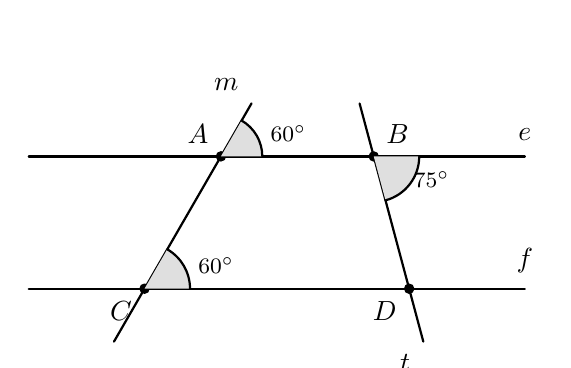
\begin{tikzpicture}[scale=1.05, line cap=round, line join=round]
    \draw[thick] (-0.8, 1.6) -- (5.2, 1.6) node[above=2pt] {$e$};
    \draw[thick] (-0.8, 0) -- (5.2, 0) node[above=2pt] {$f$};
    \coordinate (C) at (0.6, 0);
    \coordinate (A) at ($(C)+(60:1.848)$);
    \draw[thick] ($(C)!1.4!(A)$) node[above left=1pt] {$m$} -- ($(A)!1.4!(C)$);
    \coordinate (D) at (3.8, 0);
    \coordinate (B) at ($(D)+(105:1.656)$);
    \draw[thick] ($(D)!1.4!(B)$) -- ($(B)!1.4!(D)$) node[below left=1pt] {$t$};
    \filldraw[black] (A) circle (1.6pt) node[above left=1pt] {$A$};
    \filldraw[black] (C) circle (1.6pt) node[below left=1pt] {$C$};
    \filldraw[black] (B) circle (1.6pt) node[above right=1pt] {$B$};
    \filldraw[black] (D) circle (1.6pt) node[below left=1pt] {$D$};
    \fill[gray!25] (A) -- ++(0:0.5) arc (0:60:0.5) -- cycle;
    \draw[thick] (A) ++(0:0.5) arc (0:60:0.5);
    \node[font=\footnotesize, right=1pt] at ($(A)+(0.45, 0.28)$) {$60^\circ$};
    \fill[gray!25] (C) -- ++(0:0.55) arc (0:60:0.55) -- cycle;
    \draw[thick] (C) ++(0:0.55) arc (0:60:0.55);
    \node[font=\footnotesize, right=1pt] at ($(C)+(0.5, 0.28)$) {$60^\circ$};
    \fill[gray!25] (B) -- ++(0:0.55) arc (0:-75:0.55) -- cycle;
    \draw[thick] (B) ++(0:0.55) arc (0:-75:0.55);
    \node[font=\footnotesize, right=2pt] at ($(B)+(0.3, -0.28)$) {$75^\circ$};
\end{tikzpicture}
}
\loigiai{
\textbf{a)} Ta có $\widehat{mAB} = \widehat{ACD} = 60^\circ$.
Mà hai góc này ở vị trí đồng vị nên $AB \parallel CD$.
Vì $AB \parallel CD$, ta có $\widehat{BDC} = \widehat{DBe} = 75^\circ$ (hai góc so le trong).
Mặt khác, $\widehat{CDt}$ và $\widehat{BDC}$ là hai góc kề bù nên:
\[ \widehat{CDt} + \widehat{BDC} = 180^\circ \implies \widehat{CDt} = 180^\circ - 75^\circ = 105^\circ. \]

\textbf{b)} Vì $Ax$ là tia phân giác của $\widehat{mAB}$ nên $\widehat{xAB} = \dfrac{1}{2}\widehat{mAB} = \dfrac{1}{2} \cdot 60^\circ = 30^\circ$.
Vì $Cy$ là tia phân giác của $\widehat{ACD}$ nên $\widehat{yCD} = \dfrac{1}{2}\widehat{ACD} = \dfrac{1}{2} \cdot 60^\circ = 30^\circ$.
Suy ra $\widehat{xAB} = \widehat{yCD} = 30^\circ$.
Mà hai góc này ở vị trí đồng vị nên $Ax \parallel Cy$.

}
\end{ex}
\vspace{1.5mm}

\begin{ex}
Cho $M = \dfrac{1}{4} + \dfrac{1}{3^2} + \dfrac{1}{3^4} + \dfrac{1}{3^6} + \dots + \dfrac{1}{3^{802}}$. Chứng minh rằng $M < \dfrac{3}{8}$.
\loigiai{
Đặt $S = \dfrac{1}{3^2} + \dfrac{1}{3^4} + \dfrac{1}{3^6} + \dots + \dfrac{1}{3^{802}}$.
Nhân cả hai vế với $3^2 = 9$, ta được:
\[ 9S = 1 + \dfrac{1}{3^2} + \dfrac{1}{3^4} + \dots + \dfrac{1}{3^{800}}. \]
Lấy $9S - S$, ta có:
\[ 8S = 1 - \dfrac{1}{3^{802}} < 1 \implies S < \dfrac{1}{8}. \]
Khi đó:
\[ M = \dfrac{1}{4} + S < \dfrac{1}{4} + \dfrac{1}{8} = \dfrac{2}{8} + \dfrac{1}{8} = \dfrac{3}{8}. \]
Vậy $M < \dfrac{3}{8}$ (điều phải chứng minh).
}
\end{ex}
\vspace{1.5mm}


\begin{center}
\rule{4cm}{0.4pt}\\
\textit{--- HẾT ---}
\end{center}
\end{document}
